% Options for packages loaded elsewhere
\PassOptionsToPackage{unicode}{hyperref}
\PassOptionsToPackage{hyphens}{url}
%
\documentclass[
]{article}
\usepackage{amsmath,amssymb}
\usepackage{iftex}
\ifPDFTeX
  \usepackage[T1]{fontenc}
  \usepackage[utf8]{inputenc}
  \usepackage{textcomp} % provide euro and other symbols
\else % if luatex or xetex
  \usepackage{unicode-math} % this also loads fontspec
  \defaultfontfeatures{Scale=MatchLowercase}
  \defaultfontfeatures[\rmfamily]{Ligatures=TeX,Scale=1}
\fi
\usepackage{lmodern}
\ifPDFTeX\else
  % xetex/luatex font selection
\fi
% Use upquote if available, for straight quotes in verbatim environments
\IfFileExists{upquote.sty}{\usepackage{upquote}}{}
\IfFileExists{microtype.sty}{% use microtype if available
  \usepackage[]{microtype}
  \UseMicrotypeSet[protrusion]{basicmath} % disable protrusion for tt fonts
}{}
\makeatletter
\@ifundefined{KOMAClassName}{% if non-KOMA class
  \IfFileExists{parskip.sty}{%
    \usepackage{parskip}
  }{% else
    \setlength{\parindent}{0pt}
    \setlength{\parskip}{6pt plus 2pt minus 1pt}}
}{% if KOMA class
  \KOMAoptions{parskip=half}}
\makeatother
\usepackage{xcolor}
\usepackage[margin=1in]{geometry}
\usepackage{color}
\usepackage{fancyvrb}
\newcommand{\VerbBar}{|}
\newcommand{\VERB}{\Verb[commandchars=\\\{\}]}
\DefineVerbatimEnvironment{Highlighting}{Verbatim}{commandchars=\\\{\}}
% Add ',fontsize=\small' for more characters per line
\usepackage{framed}
\definecolor{shadecolor}{RGB}{248,248,248}
\newenvironment{Shaded}{\begin{snugshade}}{\end{snugshade}}
\newcommand{\AlertTok}[1]{\textcolor[rgb]{0.94,0.16,0.16}{#1}}
\newcommand{\AnnotationTok}[1]{\textcolor[rgb]{0.56,0.35,0.01}{\textbf{\textit{#1}}}}
\newcommand{\AttributeTok}[1]{\textcolor[rgb]{0.13,0.29,0.53}{#1}}
\newcommand{\BaseNTok}[1]{\textcolor[rgb]{0.00,0.00,0.81}{#1}}
\newcommand{\BuiltInTok}[1]{#1}
\newcommand{\CharTok}[1]{\textcolor[rgb]{0.31,0.60,0.02}{#1}}
\newcommand{\CommentTok}[1]{\textcolor[rgb]{0.56,0.35,0.01}{\textit{#1}}}
\newcommand{\CommentVarTok}[1]{\textcolor[rgb]{0.56,0.35,0.01}{\textbf{\textit{#1}}}}
\newcommand{\ConstantTok}[1]{\textcolor[rgb]{0.56,0.35,0.01}{#1}}
\newcommand{\ControlFlowTok}[1]{\textcolor[rgb]{0.13,0.29,0.53}{\textbf{#1}}}
\newcommand{\DataTypeTok}[1]{\textcolor[rgb]{0.13,0.29,0.53}{#1}}
\newcommand{\DecValTok}[1]{\textcolor[rgb]{0.00,0.00,0.81}{#1}}
\newcommand{\DocumentationTok}[1]{\textcolor[rgb]{0.56,0.35,0.01}{\textbf{\textit{#1}}}}
\newcommand{\ErrorTok}[1]{\textcolor[rgb]{0.64,0.00,0.00}{\textbf{#1}}}
\newcommand{\ExtensionTok}[1]{#1}
\newcommand{\FloatTok}[1]{\textcolor[rgb]{0.00,0.00,0.81}{#1}}
\newcommand{\FunctionTok}[1]{\textcolor[rgb]{0.13,0.29,0.53}{\textbf{#1}}}
\newcommand{\ImportTok}[1]{#1}
\newcommand{\InformationTok}[1]{\textcolor[rgb]{0.56,0.35,0.01}{\textbf{\textit{#1}}}}
\newcommand{\KeywordTok}[1]{\textcolor[rgb]{0.13,0.29,0.53}{\textbf{#1}}}
\newcommand{\NormalTok}[1]{#1}
\newcommand{\OperatorTok}[1]{\textcolor[rgb]{0.81,0.36,0.00}{\textbf{#1}}}
\newcommand{\OtherTok}[1]{\textcolor[rgb]{0.56,0.35,0.01}{#1}}
\newcommand{\PreprocessorTok}[1]{\textcolor[rgb]{0.56,0.35,0.01}{\textit{#1}}}
\newcommand{\RegionMarkerTok}[1]{#1}
\newcommand{\SpecialCharTok}[1]{\textcolor[rgb]{0.81,0.36,0.00}{\textbf{#1}}}
\newcommand{\SpecialStringTok}[1]{\textcolor[rgb]{0.31,0.60,0.02}{#1}}
\newcommand{\StringTok}[1]{\textcolor[rgb]{0.31,0.60,0.02}{#1}}
\newcommand{\VariableTok}[1]{\textcolor[rgb]{0.00,0.00,0.00}{#1}}
\newcommand{\VerbatimStringTok}[1]{\textcolor[rgb]{0.31,0.60,0.02}{#1}}
\newcommand{\WarningTok}[1]{\textcolor[rgb]{0.56,0.35,0.01}{\textbf{\textit{#1}}}}
\usepackage{graphicx}
\makeatletter
\def\maxwidth{\ifdim\Gin@nat@width>\linewidth\linewidth\else\Gin@nat@width\fi}
\def\maxheight{\ifdim\Gin@nat@height>\textheight\textheight\else\Gin@nat@height\fi}
\makeatother
% Scale images if necessary, so that they will not overflow the page
% margins by default, and it is still possible to overwrite the defaults
% using explicit options in \includegraphics[width, height, ...]{}
\setkeys{Gin}{width=\maxwidth,height=\maxheight,keepaspectratio}
% Set default figure placement to htbp
\makeatletter
\def\fps@figure{htbp}
\makeatother
\setlength{\emergencystretch}{3em} % prevent overfull lines
\providecommand{\tightlist}{%
  \setlength{\itemsep}{0pt}\setlength{\parskip}{0pt}}
\setcounter{secnumdepth}{-\maxdimen} % remove section numbering
\ifLuaTeX
  \usepackage{selnolig}  % disable illegal ligatures
\fi
\IfFileExists{bookmark.sty}{\usepackage{bookmark}}{\usepackage{hyperref}}
\IfFileExists{xurl.sty}{\usepackage{xurl}}{} % add URL line breaks if available
\urlstyle{same}
\hypersetup{
  pdftitle={covar-corr-demonstrations},
  pdfauthor={Sean Maden},
  hidelinks,
  pdfcreator={LaTeX via pandoc}}

\title{covar-corr-demonstrations}
\author{Sean Maden}
\date{2023-07-26}

\begin{document}
\maketitle

This notebook compares properties of two types of cell scale
transformations. For details about the transformation definitions and
derivation of the dynamic transform, see the notebook
\texttt{covar-corr-demonstrations.rmd}.

\hypertarget{load-datasets}{%
\section{Load datasets}\label{load-datasets}}

Random variables x1, y1.

\begin{Shaded}
\begin{Highlighting}[]
\CommentTok{\# get starting variables}
\NormalTok{x1 }\OtherTok{\textless{}{-}} \FunctionTok{rnbinom}\NormalTok{(}\AttributeTok{n =} \DecValTok{10}\NormalTok{, }\AttributeTok{size =} \DecValTok{10}\NormalTok{, }\AttributeTok{mu =} \DecValTok{10}\NormalTok{)  }\CommentTok{\#sample(10)}
\NormalTok{y1 }\OtherTok{\textless{}{-}} \FunctionTok{rnbinom}\NormalTok{(}\AttributeTok{n =} \DecValTok{10}\NormalTok{, }\AttributeTok{size =} \DecValTok{10}\NormalTok{, }\AttributeTok{mu =} \DecValTok{10}\NormalTok{) }\CommentTok{\#sample(10)}
\end{Highlighting}
\end{Shaded}

Cohort 1

\begin{Shaded}
\begin{Highlighting}[]
\NormalTok{base.path }\OtherTok{\textless{}{-}} \FunctionTok{file.path}\NormalTok{(}\StringTok{"outputs"}\NormalTok{, }\StringTok{"01\_prepare{-}datasets"}\NormalTok{)}
\NormalTok{sce1.filename }\OtherTok{\textless{}{-}} \StringTok{"list{-}scef\_markers{-}k2{-}k3{-}k4\_ro1{-}dlpfc.rda"}
\NormalTok{sce1.path }\OtherTok{\textless{}{-}} \FunctionTok{here}\NormalTok{(base.path, sce1.filename)}
\NormalTok{sce1 }\OtherTok{\textless{}{-}} \FunctionTok{get}\NormalTok{(}\FunctionTok{load}\NormalTok{(sce1.path))[[}\DecValTok{1}\NormalTok{]]}
\end{Highlighting}
\end{Shaded}

Cohort 2

\begin{Shaded}
\begin{Highlighting}[]
\NormalTok{sce2.filename }\OtherTok{\textless{}{-}} \StringTok{"sce{-}mrb\_dlpfc.rda"}
\NormalTok{sce2.path }\OtherTok{\textless{}{-}} \FunctionTok{here}\NormalTok{(base.path, sce2.filename)}
\NormalTok{sce2 }\OtherTok{\textless{}{-}} \FunctionTok{get}\NormalTok{(}\FunctionTok{load}\NormalTok{(sce2.path))}
\NormalTok{sce2 }\OtherTok{\textless{}{-}}\NormalTok{ sce2[}\FunctionTok{rownames}\NormalTok{(sce2) }\SpecialCharTok{\%in\%} \FunctionTok{rownames}\NormalTok{(sce1),]}
\end{Highlighting}
\end{Shaded}

\hypertarget{define-transformations}{%
\section{Define transformations}\label{define-transformations}}

Static tranformation -- this is the provided s.set series.

\begin{Shaded}
\begin{Highlighting}[]
\NormalTok{X }\OtherTok{\textless{}{-}} \DecValTok{10}
\NormalTok{Y }\OtherTok{\textless{}{-}} \DecValTok{3}
\end{Highlighting}
\end{Shaded}

Dynamic transformation -- this is a function of the starting expression
values as well as provided s.set series.

\begin{Shaded}
\begin{Highlighting}[]
\NormalTok{adj.weight.x }\OtherTok{\textless{}{-}} \ControlFlowTok{function}\NormalTok{(WeightX, WeightY, x1, y1, }\AttributeTok{offset=}\FloatTok{1e{-}5}\NormalTok{)\{}
  \CommentTok{\# Transform x and y such that their correlation decreases, and their covariance remains negative?}
  \CommentTok{\# x1 : first cell type}
  \CommentTok{\# y1 : second cell type}
\NormalTok{  fract }\OtherTok{\textless{}{-}}\NormalTok{ WeightX}\SpecialCharTok{/}\NormalTok{WeightY}
\NormalTok{  (fract}\SpecialCharTok{*}\NormalTok{y1}\SpecialCharTok{*}\NormalTok{WeightY}\SpecialCharTok{+}\NormalTok{offset)}\SpecialCharTok{/}\NormalTok{(x1}\SpecialCharTok{+}\NormalTok{offset)}
\NormalTok{\}}
\NormalTok{get.adj }\OtherTok{\textless{}{-}} \ControlFlowTok{function}\NormalTok{(x1, y1, WeightX, WeightY)\{}
  \CommentTok{\# pseudoalgorithm}
  \CommentTok{\# given a vector of normalizations, get the fraction, x/y}
  \CommentTok{\# now adjust vectors x1, y1 such that the ratio is achieved}
\NormalTok{  X.adj }\OtherTok{\textless{}{-}} \FunctionTok{adj.weight.x}\NormalTok{(}\AttributeTok{WeightX =}\NormalTok{ WeightX, }\AttributeTok{WeightY =}\NormalTok{ WeightY, }\AttributeTok{x1 =}\NormalTok{ x1, }\AttributeTok{y1 =}\NormalTok{ y1)}
\NormalTok{  Y.adj }\OtherTok{\textless{}{-}} \FunctionTok{adj.weight.x}\NormalTok{(}\AttributeTok{WeightX =}\NormalTok{ WeightY, }\AttributeTok{WeightY =}\NormalTok{ WeightX, }\AttributeTok{x1 =}\NormalTok{ x1, }\AttributeTok{y1 =}\NormalTok{ y1)}
  \FunctionTok{list}\NormalTok{(}\AttributeTok{x.adj=}\NormalTok{x1}\SpecialCharTok{*}\NormalTok{X.adj, }\AttributeTok{y.adj=}\NormalTok{y1}\SpecialCharTok{*}\NormalTok{Y.adj)}
\NormalTok{\}}
\end{Highlighting}
\end{Shaded}

\begin{Shaded}
\begin{Highlighting}[]
\CommentTok{\# CRITICALITY CHECK: for identical terms (x1==y1), expect X.adj==X, Y.adj==Y}
\NormalTok{X.adj }\OtherTok{\textless{}{-}} \FunctionTok{adj.weight.x}\NormalTok{(}\AttributeTok{WeightX =}\NormalTok{ X, }\AttributeTok{WeightY =}\NormalTok{ Y, }\AttributeTok{x1 =}\NormalTok{ x1[}\DecValTok{1}\NormalTok{], }\AttributeTok{y1 =}\NormalTok{ y1[}\DecValTok{1}\NormalTok{])}
\NormalTok{Y.adj }\OtherTok{\textless{}{-}} \FunctionTok{adj.weight.x}\NormalTok{(}\AttributeTok{WeightX =}\NormalTok{ Y, }\AttributeTok{WeightY =}\NormalTok{ X, }\AttributeTok{x1 =}\NormalTok{ x1[}\DecValTok{1}\NormalTok{], }\AttributeTok{y1 =}\NormalTok{ y1[}\DecValTok{1}\NormalTok{])}
\FunctionTok{round}\NormalTok{(X.adj)}\SpecialCharTok{==}\NormalTok{X}
\end{Highlighting}
\end{Shaded}

\begin{verbatim}
## [1] TRUE
\end{verbatim}

\begin{Shaded}
\begin{Highlighting}[]
\FunctionTok{round}\NormalTok{(Y.adj)}\SpecialCharTok{==}\NormalTok{Y}
\end{Highlighting}
\end{Shaded}

\begin{verbatim}
## [1] TRUE
\end{verbatim}

\hypertarget{compare-static-vs-dynamic}{%
\section{Compare static vs dynamic}\label{compare-static-vs-dynamic}}

\begin{Shaded}
\begin{Highlighting}[]
\NormalTok{adj.xy }\OtherTok{\textless{}{-}} \FunctionTok{get.adj}\NormalTok{(x1, y1, }\AttributeTok{WeightX =}\NormalTok{ X, }\AttributeTok{WeightY =}\NormalTok{ Y)}
\NormalTok{x2 }\OtherTok{\textless{}{-}}\NormalTok{ adj.xy[[}\DecValTok{1}\NormalTok{]]}
\NormalTok{y2 }\OtherTok{\textless{}{-}}\NormalTok{ adj.xy[[}\DecValTok{2}\NormalTok{]]}
\NormalTok{dfp }\OtherTok{\textless{}{-}} \FunctionTok{rbind}\NormalTok{(}\FunctionTok{data.frame}\NormalTok{(}\AttributeTok{x =}\NormalTok{ x1, }\AttributeTok{y =}\NormalTok{ y1, }\AttributeTok{type =} \FunctionTok{rep}\NormalTok{(}\StringTok{"unadj"}\NormalTok{, }\FunctionTok{length}\NormalTok{(x1))),}
             \FunctionTok{data.frame}\NormalTok{(}\AttributeTok{x =}\NormalTok{ x2, }\AttributeTok{y =}\NormalTok{ y2, }\AttributeTok{type =} \FunctionTok{rep}\NormalTok{(}\StringTok{"dynamic"}\NormalTok{, }\FunctionTok{length}\NormalTok{(x2))))}
\NormalTok{dfp }\OtherTok{\textless{}{-}} \FunctionTok{rbind}\NormalTok{(dfp, }\FunctionTok{data.frame}\NormalTok{(}\AttributeTok{x =}\NormalTok{ x1}\SpecialCharTok{*}\NormalTok{X, }\AttributeTok{y =}\NormalTok{ y1}\SpecialCharTok{*}\NormalTok{Y, }\AttributeTok{type =} \FunctionTok{rep}\NormalTok{(}\StringTok{"static"}\NormalTok{, }\FunctionTok{length}\NormalTok{(x1))))}
\FunctionTok{ggplot}\NormalTok{(dfp, }\FunctionTok{aes}\NormalTok{(}\AttributeTok{x =}\NormalTok{ x, }\AttributeTok{y =}\NormalTok{ y, }\AttributeTok{color =}\NormalTok{ type)) }\SpecialCharTok{+} \FunctionTok{geom\_point}\NormalTok{() }\SpecialCharTok{+} \FunctionTok{facet\_wrap}\NormalTok{(}\SpecialCharTok{\textasciitilde{}}\NormalTok{type) }\SpecialCharTok{+}
  \FunctionTok{geom\_abline}\NormalTok{(}\AttributeTok{slope =} \DecValTok{1}\NormalTok{, }\AttributeTok{intercept =} \DecValTok{0}\NormalTok{) }\SpecialCharTok{+} \FunctionTok{ggtitle}\NormalTok{(}\StringTok{"Marker expression"}\NormalTok{)}
\end{Highlighting}
\end{Shaded}

\includegraphics{sset-static-vs-dynamic_cohorts-1-2_files/figure-latex/unnamed-chunk-7-1.pdf}

\begin{Shaded}
\begin{Highlighting}[]
\CommentTok{\# cor tests}
\CommentTok{\# unadj}
\FunctionTok{cor}\NormalTok{(dfp[dfp}\SpecialCharTok{$}\NormalTok{type}\SpecialCharTok{==}\StringTok{"unadj"}\NormalTok{,]}\SpecialCharTok{$}\NormalTok{x,dfp[dfp}\SpecialCharTok{$}\NormalTok{type}\SpecialCharTok{==}\StringTok{"unadj"}\NormalTok{,]}\SpecialCharTok{$}\NormalTok{y) }\CommentTok{\# {-}0.2988827}
\end{Highlighting}
\end{Shaded}

\begin{verbatim}
## [1] -0.2988827
\end{verbatim}

\begin{Shaded}
\begin{Highlighting}[]
\CommentTok{\# static}
\FunctionTok{cor}\NormalTok{(dfp[dfp}\SpecialCharTok{$}\NormalTok{type}\SpecialCharTok{==}\StringTok{"static"}\NormalTok{,]}\SpecialCharTok{$}\NormalTok{x,dfp[dfp}\SpecialCharTok{$}\NormalTok{type}\SpecialCharTok{==}\StringTok{"static"}\NormalTok{,]}\SpecialCharTok{$}\NormalTok{y) }\CommentTok{\# {-}0.2988827}
\end{Highlighting}
\end{Shaded}

\begin{verbatim}
## [1] -0.2988827
\end{verbatim}

\begin{Shaded}
\begin{Highlighting}[]
\CommentTok{\# dynamic}
\FunctionTok{cor}\NormalTok{(dfp[dfp}\SpecialCharTok{$}\NormalTok{type}\SpecialCharTok{==}\StringTok{"dynamic"}\NormalTok{,]}\SpecialCharTok{$}\NormalTok{x,dfp[dfp}\SpecialCharTok{$}\NormalTok{type}\SpecialCharTok{==}\StringTok{"dynamic"}\NormalTok{,]}\SpecialCharTok{$}\NormalTok{y) }\CommentTok{\# [1] 0.9354588}
\end{Highlighting}
\end{Shaded}

\begin{verbatim}
## [1] 0.9354587
\end{verbatim}

\begin{Shaded}
\begin{Highlighting}[]
\CommentTok{\# cov tests}
\CommentTok{\# unadj}
\FunctionTok{cov}\NormalTok{(dfp[dfp}\SpecialCharTok{$}\NormalTok{type}\SpecialCharTok{==}\StringTok{"unadj"}\NormalTok{,]}\SpecialCharTok{$}\NormalTok{x,dfp[dfp}\SpecialCharTok{$}\NormalTok{type}\SpecialCharTok{==}\StringTok{"unadj"}\NormalTok{,]}\SpecialCharTok{$}\NormalTok{y) }\CommentTok{\# {-}3.7}
\end{Highlighting}
\end{Shaded}

\begin{verbatim}
## [1] -3.7
\end{verbatim}

\begin{Shaded}
\begin{Highlighting}[]
\CommentTok{\# static}
\FunctionTok{cov}\NormalTok{(dfp[dfp}\SpecialCharTok{$}\NormalTok{type}\SpecialCharTok{==}\StringTok{"static"}\NormalTok{,]}\SpecialCharTok{$}\NormalTok{x,dfp[dfp}\SpecialCharTok{$}\NormalTok{type}\SpecialCharTok{==}\StringTok{"static"}\NormalTok{,]}\SpecialCharTok{$}\NormalTok{y) }\CommentTok{\# {-}111}
\end{Highlighting}
\end{Shaded}

\begin{verbatim}
## [1] -111
\end{verbatim}

\begin{Shaded}
\begin{Highlighting}[]
\CommentTok{\# dynamic}
\FunctionTok{cov}\NormalTok{(dfp[dfp}\SpecialCharTok{$}\NormalTok{type}\SpecialCharTok{==}\StringTok{"dynamic"}\NormalTok{,]}\SpecialCharTok{$}\NormalTok{x,dfp[dfp}\SpecialCharTok{$}\NormalTok{type}\SpecialCharTok{==}\StringTok{"dynamic"}\NormalTok{,]}\SpecialCharTok{$}\NormalTok{y) }\CommentTok{\# 1093.662}
\end{Highlighting}
\end{Shaded}

\begin{verbatim}
## [1] 1093.659
\end{verbatim}

\hypertarget{compare-static-vs-dynamic-mrb-cohort2-dataset}{%
\section{Compare static vs dynamic -- mrb cohort2
dataset}\label{compare-static-vs-dynamic-mrb-cohort2-dataset}}

\begin{Shaded}
\begin{Highlighting}[]
\NormalTok{z.unadj }\OtherTok{\textless{}{-}}\NormalTok{ lute}\SpecialCharTok{:::}\FunctionTok{.get\_z\_from\_sce}\NormalTok{(sce2, }\StringTok{"counts"}\NormalTok{, }\StringTok{"k2"}\NormalTok{)}

\NormalTok{z.static }\OtherTok{\textless{}{-}}\NormalTok{ lute}\SpecialCharTok{:::}\FunctionTok{.get\_z\_from\_sce}\NormalTok{(sce2, }\StringTok{"counts"}\NormalTok{, }\StringTok{"k2"}\NormalTok{) }\SpecialCharTok{\%\textgreater{}\%}
\NormalTok{  lute}\SpecialCharTok{:::}\FunctionTok{.zstransform}\NormalTok{(}\AttributeTok{s =} \FunctionTok{c}\NormalTok{(}\StringTok{"glial"} \OtherTok{=} \DecValTok{3}\NormalTok{, }\StringTok{"neuron"} \OtherTok{=} \DecValTok{10}\NormalTok{))}

\NormalTok{ladj }\OtherTok{\textless{}{-}} \FunctionTok{get.adj}\NormalTok{(}\AttributeTok{x1 =}\NormalTok{ z.unadj[,}\DecValTok{1}\NormalTok{], }\AttributeTok{y1 =}\NormalTok{ z.unadj[,}\DecValTok{2}\NormalTok{], }\AttributeTok{WeightX =} \DecValTok{3}\NormalTok{, }\AttributeTok{WeightY =} \DecValTok{10}\NormalTok{)}

\NormalTok{z.dynamic }\OtherTok{\textless{}{-}} \FunctionTok{do.call}\NormalTok{(cbind, }\FunctionTok{lapply}\NormalTok{(ladj, }\ControlFlowTok{function}\NormalTok{(type.expr)\{type.expr\}))}
\FunctionTok{colnames}\NormalTok{(z.dynamic) }\OtherTok{\textless{}{-}} \FunctionTok{c}\NormalTok{(}\StringTok{"glial"}\NormalTok{, }\StringTok{"neuron"}\NormalTok{)}
\end{Highlighting}
\end{Shaded}

\begin{Shaded}
\begin{Highlighting}[]
\NormalTok{dfp }\OtherTok{\textless{}{-}} \FunctionTok{rbind}\NormalTok{(}
  \FunctionTok{data.frame}\NormalTok{(}\AttributeTok{neuron =}\NormalTok{ z.unadj[,}\StringTok{"neuron"}\NormalTok{], }\AttributeTok{glial =}\NormalTok{ z.unadj[,}\StringTok{"glial"}\NormalTok{], }\AttributeTok{type =} \FunctionTok{rep}\NormalTok{(}\StringTok{"unadj"}\NormalTok{, }\FunctionTok{nrow}\NormalTok{(z.unadj))),}
  \FunctionTok{data.frame}\NormalTok{(}\AttributeTok{neuron =}\NormalTok{ z.static[,}\StringTok{"neuron"}\NormalTok{], }\AttributeTok{glial =}\NormalTok{ z.static[,}\StringTok{"glial"}\NormalTok{], }\AttributeTok{type =} \FunctionTok{rep}\NormalTok{(}\StringTok{"static"}\NormalTok{, }\FunctionTok{nrow}\NormalTok{(z.static)))}
\NormalTok{)}
\NormalTok{dfp }\OtherTok{\textless{}{-}} \FunctionTok{rbind}\NormalTok{(dfp,}
             \FunctionTok{data.frame}\NormalTok{(}
               \AttributeTok{neuron =}\NormalTok{ z.dynamic[,}\StringTok{"neuron"}\NormalTok{], }\AttributeTok{glial =}\NormalTok{ z.dynamic[,}\StringTok{"glial"}\NormalTok{], }
               \AttributeTok{type =} \FunctionTok{rep}\NormalTok{(}\StringTok{"dynamic"}\NormalTok{, }\FunctionTok{nrow}\NormalTok{(z.dynamic))))}

\FunctionTok{ggplot}\NormalTok{(dfp, }\FunctionTok{aes}\NormalTok{(}\AttributeTok{x =}\NormalTok{ neuron, }\AttributeTok{y =}\NormalTok{ glial, }\AttributeTok{color =}\NormalTok{ type)) }\SpecialCharTok{+} 
  \FunctionTok{geom\_point}\NormalTok{() }\SpecialCharTok{+} \FunctionTok{facet\_wrap}\NormalTok{(}\SpecialCharTok{\textasciitilde{}}\NormalTok{type) }\SpecialCharTok{+}
  \FunctionTok{geom\_abline}\NormalTok{(}\AttributeTok{slope =} \DecValTok{1}\NormalTok{, }\AttributeTok{intercept =} \DecValTok{0}\NormalTok{) }\SpecialCharTok{+}
  \FunctionTok{ggtitle}\NormalTok{(}\StringTok{"Marker expression"}\NormalTok{)}
\end{Highlighting}
\end{Shaded}

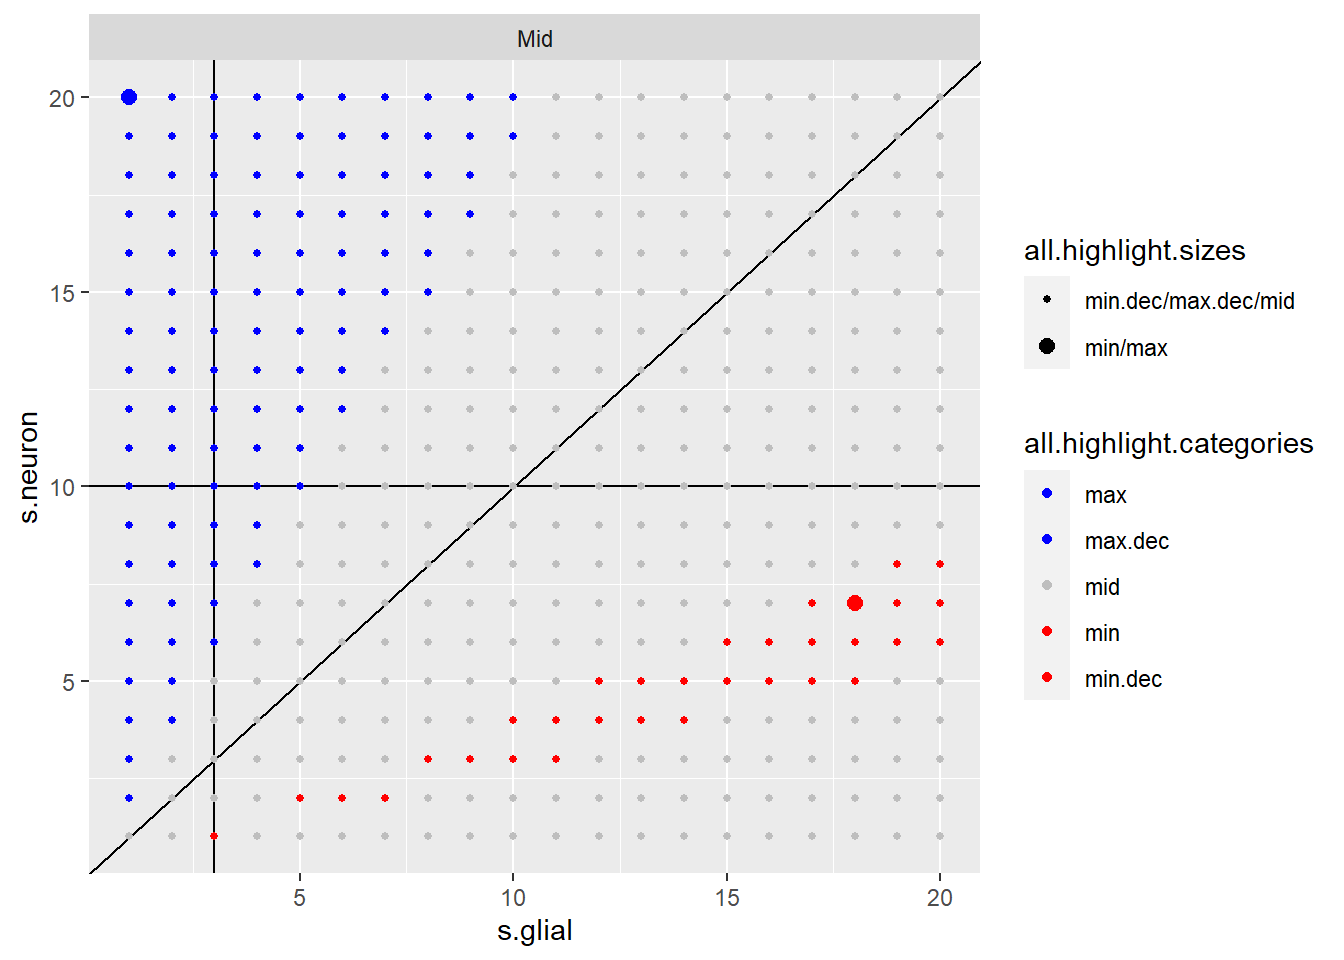
\includegraphics{sset-static-vs-dynamic_cohorts-1-2_files/figure-latex/unnamed-chunk-11-1.pdf}

\hypertarget{compare-static-vs-dynamic-dlpfc-cohort1-dataset}{%
\section{Compare static vs dynamic -- dlpfc cohort1
dataset}\label{compare-static-vs-dynamic-dlpfc-cohort1-dataset}}

\begin{Shaded}
\begin{Highlighting}[]
\CommentTok{\# get z matrices}
\NormalTok{z.unadj }\OtherTok{\textless{}{-}}\NormalTok{ lute}\SpecialCharTok{:::}\FunctionTok{.get\_z\_from\_sce}\NormalTok{(sce1, }\StringTok{"counts"}\NormalTok{, }\StringTok{"k2"}\NormalTok{)}

\NormalTok{z.static }\OtherTok{\textless{}{-}}\NormalTok{ lute}\SpecialCharTok{:::}\FunctionTok{.get\_z\_from\_sce}\NormalTok{(sce1, }\StringTok{"counts"}\NormalTok{, }\StringTok{"k2"}\NormalTok{) }\SpecialCharTok{\%\textgreater{}\%}
\NormalTok{  lute}\SpecialCharTok{:::}\FunctionTok{.zstransform}\NormalTok{(}\AttributeTok{s =} \FunctionTok{c}\NormalTok{(}\StringTok{"glial"} \OtherTok{=} \DecValTok{3}\NormalTok{, }\StringTok{"neuron"} \OtherTok{=} \DecValTok{10}\NormalTok{))}

\NormalTok{ladj }\OtherTok{\textless{}{-}} \FunctionTok{get.adj}\NormalTok{(}\AttributeTok{x1 =}\NormalTok{ z.unadj[,}\DecValTok{1}\NormalTok{], }\AttributeTok{y1 =}\NormalTok{ z.unadj[,}\DecValTok{2}\NormalTok{], }\AttributeTok{WeightX =} \DecValTok{3}\NormalTok{, }\AttributeTok{WeightY =} \DecValTok{10}\NormalTok{)}
\NormalTok{z.dynamic }\OtherTok{\textless{}{-}} \FunctionTok{do.call}\NormalTok{(cbind, }\FunctionTok{lapply}\NormalTok{(ladj, }\ControlFlowTok{function}\NormalTok{(type.expr)\{type.expr\}))}
\FunctionTok{colnames}\NormalTok{(z.dynamic) }\OtherTok{\textless{}{-}} \FunctionTok{c}\NormalTok{(}\StringTok{"glial"}\NormalTok{, }\StringTok{"neuron"}\NormalTok{)}
\end{Highlighting}
\end{Shaded}

\begin{Shaded}
\begin{Highlighting}[]
\NormalTok{dfp }\OtherTok{\textless{}{-}} \FunctionTok{rbind}\NormalTok{(}
  \FunctionTok{data.frame}\NormalTok{(}\AttributeTok{neuron =}\NormalTok{ z.unadj[,}\StringTok{"neuron"}\NormalTok{], }\AttributeTok{glial =}\NormalTok{ z.unadj[,}\StringTok{"glial"}\NormalTok{], }\AttributeTok{type =} \FunctionTok{rep}\NormalTok{(}\StringTok{"unadj"}\NormalTok{, }\FunctionTok{nrow}\NormalTok{(z.unadj))),}
  \FunctionTok{data.frame}\NormalTok{(}\AttributeTok{neuron =}\NormalTok{ z.static[,}\StringTok{"neuron"}\NormalTok{], }\AttributeTok{glial =}\NormalTok{ z.static[,}\StringTok{"glial"}\NormalTok{], }\AttributeTok{type =} \FunctionTok{rep}\NormalTok{(}\StringTok{"static"}\NormalTok{, }\FunctionTok{nrow}\NormalTok{(z.static)))}
\NormalTok{)}
\NormalTok{dfp }\OtherTok{\textless{}{-}} \FunctionTok{rbind}\NormalTok{(}
\NormalTok{  dfp,}
  \FunctionTok{data.frame}\NormalTok{(}
    \AttributeTok{neuron =}\NormalTok{ z.dynamic[,}\StringTok{"neuron"}\NormalTok{], }\AttributeTok{glial =}\NormalTok{ z.dynamic[,}\StringTok{"glial"}\NormalTok{], }
    \AttributeTok{type =} \FunctionTok{rep}\NormalTok{(}\StringTok{"dynamic"}\NormalTok{, }\FunctionTok{nrow}\NormalTok{(z.dynamic)))}
\NormalTok{)}

\FunctionTok{ggplot}\NormalTok{(dfp, }\FunctionTok{aes}\NormalTok{(}\AttributeTok{x =}\NormalTok{ neuron, }\AttributeTok{y =}\NormalTok{ glial, }\AttributeTok{color =}\NormalTok{ type)) }\SpecialCharTok{+} 
  \FunctionTok{geom\_point}\NormalTok{() }\SpecialCharTok{+} \FunctionTok{facet\_wrap}\NormalTok{(}\SpecialCharTok{\textasciitilde{}}\NormalTok{type) }\SpecialCharTok{+}
  \FunctionTok{geom\_abline}\NormalTok{(}\AttributeTok{slope =} \DecValTok{1}\NormalTok{, }\AttributeTok{intercept =} \DecValTok{0}\NormalTok{) }\SpecialCharTok{+}
  \FunctionTok{ggtitle}\NormalTok{(}\StringTok{"Marker expression"}\NormalTok{)}
\end{Highlighting}
\end{Shaded}

\includegraphics{sset-static-vs-dynamic_cohorts-1-2_files/figure-latex/unnamed-chunk-13-1.pdf}

\hypertarget{compare-bulk}{%
\section{Compare bulk}\label{compare-bulk}}

Test if linear adjustment of bulk is impacted by static or dynamic
transformation.

\begin{Shaded}
\begin{Highlighting}[]
\NormalTok{mae.filename }\OtherTok{\textless{}{-}} \StringTok{"mae\_with{-}rpkm\_additional{-}data\_final.rda"}
\NormalTok{mae.path }\OtherTok{\textless{}{-}} \FunctionTok{file.path}\NormalTok{(base.path, mae.filename)}
\NormalTok{mae }\OtherTok{\textless{}{-}} \FunctionTok{get}\NormalTok{(}\FunctionTok{load}\NormalTok{(mae.path))}
\end{Highlighting}
\end{Shaded}

Prep inputs

\begin{Shaded}
\begin{Highlighting}[]
\NormalTok{y }\OtherTok{\textless{}{-}} \FunctionTok{assays}\NormalTok{(mae[[}\StringTok{"bulk.rnaseq"}\NormalTok{]])[[}\DecValTok{1}\NormalTok{]]}
\end{Highlighting}
\end{Shaded}

\begin{verbatim}
## Loading required package: MultiAssayExperiment
\end{verbatim}

\begin{Shaded}
\begin{Highlighting}[]
\NormalTok{y }\OtherTok{\textless{}{-}}\NormalTok{ y[}\FunctionTok{rownames}\NormalTok{(z.unadj),] }\SpecialCharTok{\%\textgreater{}\%} \FunctionTok{as.matrix}\NormalTok{()}
\CommentTok{\# get lm fits}
\NormalTok{z.iter }\OtherTok{\textless{}{-}}\NormalTok{ z.unadj}
\NormalTok{zlist }\OtherTok{\textless{}{-}} \FunctionTok{list}\NormalTok{(}\AttributeTok{z.unadj =}\NormalTok{ z.unadj, }\AttributeTok{z.static =}\NormalTok{ z.static, }\AttributeTok{z.dynamic =}\NormalTok{ z.dynamic)}
\end{Highlighting}
\end{Shaded}

Perform experiment

\begin{Shaded}
\begin{Highlighting}[]
\CommentTok{\#{-}{-}{-}{-}{-}{-}{-}{-}{-}{-}{-}{-}{-}{-}{-}{-}{-}}
\CommentTok{\# get wide results}
\CommentTok{\#{-}{-}{-}{-}{-}{-}{-}{-}{-}{-}{-}{-}{-}{-}{-}{-}{-}}
\NormalTok{dfres }\OtherTok{\textless{}{-}} \FunctionTok{do.call}\NormalTok{(rbind, }\FunctionTok{lapply}\NormalTok{(}\FunctionTok{seq}\NormalTok{(}\FunctionTok{ncol}\NormalTok{(y)), }\ControlFlowTok{function}\NormalTok{(index.y)\{}
\NormalTok{  dflm }\OtherTok{\textless{}{-}} \FunctionTok{data.frame}\NormalTok{(}\AttributeTok{y.expr.counts =} \FunctionTok{as.numeric}\NormalTok{(y[,index.y]))}
  \CommentTok{\# get df of fitted values}
\NormalTok{  dffit }\OtherTok{\textless{}{-}} \FunctionTok{do.call}\NormalTok{(cbind, }\FunctionTok{lapply}\NormalTok{(}\FunctionTok{seq}\NormalTok{(}\FunctionTok{length}\NormalTok{(zlist)), }\ControlFlowTok{function}\NormalTok{(index.z)\{}
\NormalTok{    z.iter }\OtherTok{\textless{}{-}}\NormalTok{ zlist[[index.z]]}
\NormalTok{    dflm}\SpecialCharTok{$}\NormalTok{type1 }\OtherTok{\textless{}{-}}\NormalTok{ z.iter[,}\DecValTok{1}\NormalTok{]; dflm}\SpecialCharTok{$}\NormalTok{type2 }\OtherTok{\textless{}{-}}\NormalTok{ z.iter[,}\DecValTok{2}\NormalTok{]}
    \FunctionTok{lm}\NormalTok{(y.expr.counts}\SpecialCharTok{\textasciitilde{}}\NormalTok{type1}\SpecialCharTok{+}\NormalTok{type2,}\AttributeTok{data=}\NormalTok{dflm)}\SpecialCharTok{$}\NormalTok{fitted.values}
\NormalTok{  \}))}
  \CommentTok{\# format fitted results}
  \FunctionTok{colnames}\NormalTok{(dffit) }\OtherTok{\textless{}{-}} \FunctionTok{paste0}\NormalTok{(}\StringTok{"fitted."}\NormalTok{, }\FunctionTok{names}\NormalTok{(zlist))}
\NormalTok{  z.label.iter }\OtherTok{\textless{}{-}} \FunctionTok{names}\NormalTok{(zlist)}
\NormalTok{  dfr }\OtherTok{\textless{}{-}} \FunctionTok{cbind}\NormalTok{(dflm, dffit)}
\NormalTok{  dfr}\SpecialCharTok{$}\NormalTok{sample.id }\OtherTok{\textless{}{-}} \FunctionTok{colnames}\NormalTok{(y)[index.y]}
\NormalTok{  dfr}\SpecialCharTok{$}\NormalTok{marker.id }\OtherTok{\textless{}{-}} \FunctionTok{rownames}\NormalTok{(z.unadj)}
  \FunctionTok{return}\NormalTok{(dfr)}
\NormalTok{\}))}
\CommentTok{\# get differences by z type}
\NormalTok{dfres}\SpecialCharTok{$}\NormalTok{diff.z.static.unadj }\OtherTok{\textless{}{-}}\NormalTok{ dfres}\SpecialCharTok{$}\NormalTok{fitted.z.static}\SpecialCharTok{{-}}\NormalTok{dfres}\SpecialCharTok{$}\NormalTok{fitted.z.unadj}
\NormalTok{dfres}\SpecialCharTok{$}\NormalTok{diff.z.dynamic.unadj }\OtherTok{\textless{}{-}}\NormalTok{ dfres}\SpecialCharTok{$}\NormalTok{fitted.z.dynamic}\SpecialCharTok{{-}}\NormalTok{dfres}\SpecialCharTok{$}\NormalTok{fitted.z.unadj}
\NormalTok{dfwide }\OtherTok{\textless{}{-}}\NormalTok{ dfres}

\CommentTok{\#{-}{-}{-}{-}{-}{-}{-}{-}{-}{-}{-}{-}{-}{-}{-}{-}{-}}
\CommentTok{\# get tall results}
\CommentTok{\#{-}{-}{-}{-}{-}{-}{-}{-}{-}{-}{-}{-}{-}{-}{-}{-}{-}}
\CommentTok{\# dftall \textless{}{-} do.call(rbind, lapply(, function()))}
\NormalTok{dftall }\OtherTok{\textless{}{-}}\NormalTok{ reshape2}\SpecialCharTok{::}\FunctionTok{melt}\NormalTok{(dfres)}
\end{Highlighting}
\end{Shaded}

\begin{verbatim}
## Using sample.id, marker.id as id variables
\end{verbatim}

Plot results for single sample

\begin{Shaded}
\begin{Highlighting}[]
\CommentTok{\# plots the differences by z treatment}
\CommentTok{\# defines the dfp filter}
\NormalTok{dftall.filter }\OtherTok{\textless{}{-}}\NormalTok{ dftall}\SpecialCharTok{$}\NormalTok{sample.id}\SpecialCharTok{==}\StringTok{"2107UNHS{-}0291\_Br2720\_Mid\_Bulk"}
\NormalTok{dftall.filter }\OtherTok{\textless{}{-}}\NormalTok{ dftall.filter }\SpecialCharTok{\&}\NormalTok{ dftall}\SpecialCharTok{$}\NormalTok{variable }\SpecialCharTok{\%in\%} \FunctionTok{c}\NormalTok{(}\StringTok{"diff.z.static.unadj"}\NormalTok{, }\StringTok{"diff.z.dynamic.unadj"}\NormalTok{)}
\NormalTok{dfp.new }\OtherTok{\textless{}{-}}\NormalTok{ dftall[dftall.filter,]}
\FunctionTok{ggplot}\NormalTok{(dfp.new, }\FunctionTok{aes}\NormalTok{(}\AttributeTok{x =}\NormalTok{ variable, }\AttributeTok{y =}\NormalTok{ value)) }\SpecialCharTok{+} \FunctionTok{geom\_jitter}\NormalTok{() }\SpecialCharTok{+} \FunctionTok{geom\_boxplot}\NormalTok{(}\AttributeTok{alpha =} \DecValTok{0}\NormalTok{) }\SpecialCharTok{+} \FunctionTok{facet\_wrap}\NormalTok{(}\SpecialCharTok{\textasciitilde{}}\NormalTok{sample.id)}
\end{Highlighting}
\end{Shaded}

\includegraphics{sset-static-vs-dynamic_cohorts-1-2_files/figure-latex/unnamed-chunk-17-1.pdf}

\begin{Shaded}
\begin{Highlighting}[]
\CommentTok{\# plots scatterplot of adj diffs by marker }
\NormalTok{dfwide.filter }\OtherTok{\textless{}{-}}\NormalTok{ dfwide}\SpecialCharTok{$}\NormalTok{sample.id}\SpecialCharTok{==}\StringTok{"2107UNHS{-}0291\_Br2720\_Mid\_Bulk"}
\NormalTok{dfp.new }\OtherTok{\textless{}{-}}\NormalTok{ dfwide[dfwide.filter,]}
\FunctionTok{ggplot}\NormalTok{(dfp.new, }\FunctionTok{aes}\NormalTok{(}\AttributeTok{x =}\NormalTok{ diff.z.static.unadj, }\AttributeTok{y =}\NormalTok{ diff.z.dynamic.unadj)) }\SpecialCharTok{+} 
  \FunctionTok{geom\_jitter}\NormalTok{() }\SpecialCharTok{+} \FunctionTok{geom\_point}\NormalTok{() }\SpecialCharTok{+} \FunctionTok{geom\_abline}\NormalTok{(}\AttributeTok{slope =} \DecValTok{1}\NormalTok{, }\AttributeTok{intercept =} \DecValTok{0}\NormalTok{) }\SpecialCharTok{+}
  \FunctionTok{geom\_text}\NormalTok{(}\FunctionTok{aes}\NormalTok{(}\AttributeTok{label =}\NormalTok{ marker.id))}
\end{Highlighting}
\end{Shaded}

\includegraphics{sset-static-vs-dynamic_cohorts-1-2_files/figure-latex/unnamed-chunk-17-2.pdf}

\begin{Shaded}
\begin{Highlighting}[]
\CommentTok{\# ggpairs for marker expression}
\NormalTok{colnames.filter }\OtherTok{\textless{}{-}} \FunctionTok{c}\NormalTok{(}\StringTok{"fitted.z.unadj"}\NormalTok{, }\StringTok{"fitted.z.static"}\NormalTok{, }\StringTok{"fitted.z.dynamic"}\NormalTok{)}
\FunctionTok{pairs}\NormalTok{(dfwide[,colnames.filter])}
\end{Highlighting}
\end{Shaded}

\includegraphics{sset-static-vs-dynamic_cohorts-1-2_files/figure-latex/unnamed-chunk-17-3.pdf}

\end{document}
